%% Простая презентация с примером включения программного кода и
%% пошаговых спецэффектов
\documentclass{beamer}
\usetheme{SPbAU}
%\useoutertheme{infolines}
\usepackage{fontspec}
\usepackage{xunicode}
\usepackage{xltxtra}
\usepackage{xecyr}
\usepackage{hyperref}
\setmainfont[Mapping=tex-text]{DejaVu Serif}
\setsansfont[Mapping=tex-text]{DejaVu Sans}
\setmonofont[Mapping=tex-text]{DejaVu Sans Mono}
\usepackage{polyglossia}
\usepackage{csquotes}
\setdefaultlanguage{russian}
\usepackage{graphicx}
\usepackage{listings}
\usepackage{xpatch}
\usepackage{minted}
\usepackage{tikz}
\usepackage{float}
\usepackage[noend]{algpseudocode}
\usepackage{algorithm}
\usepackage{caption}
\usepackage{changepage}
\usetikzlibrary{tikzmark}
\lstdefinestyle{highlight}{
  basicstyle=\footnotesize\ttfamily\color{black},
  keywordstyle=\bfseries\color{black},
  commentstyle=\itshape\color{black},
}
\lstdefinestyle{base}{
  belowcaptionskip=1\baselineskip,
  breaklines=true,
  xleftmargin=\parindent,
  showstringspaces=false,
  basicstyle=\footnotesize\ttfamily\color{black!40},
  keywordstyle=\bfseries\color{black!40},
  commentstyle=\ttfamily\itshape\color{black!40},
  stringstyle=\color{red},
  numbers=left,
  numbersep=5pt,
  numberstyle=\tiny\color{gray},
  morecomment=[s]{(*}{*)},
  texcl=true,
  literate={п}{\cyrp}1
             {и}{\cyri}1,
  moredelim=**[is][\only<+>{\color{black}\lstset{style=highlight}}]{§}{§},
  morekeywords={implicit, module, struct, sig, val}
}
\lstdefinestyle{base2}{
  belowcaptionskip=1\baselineskip,
  breaklines=true,
  xleftmargin=\parindent,
  showstringspaces=false,
  basicstyle=\footnotesize\ttfamily\color{black},
  keywordstyle=\bfseries\color{black},
  commentstyle=\ttfamily\itshape\color{black},
  stringstyle=\color{red},
  numbers=left,
  numbersep=5pt,
  numberstyle=\tiny\color{gray},
  morecomment=[l]{(*},
  texcl=true,
  literate={п}{\cyrp}1
             {и}{\cyri}1,
  moredelim=**[is][\only<+>{\color{black}\lstset{style=highlight}}]{§}{§},
  morekeywords={implicit, module, struct, sig, val}
}
\newcommand{\backupbegin}{
   \newcounter{framenumberappendix}
   \setcounter{framenumberappendix}{\value{framenumber}}
}
\newcommand{\backupend}{
   \addtocounter{framenumberappendix}{-\value{framenumber}}
   \addtocounter{framenumber}{\value{framenumberappendix}} 
}
\usepackage[backend=biber, style=authortitle, doi=false, url=false, isbn=false]{biblatex}
\xapptobibmacro{cite}{\setunit{\nametitledelim}}{}{}
\renewbibmacro*{cite:title}{%
  \printtext[bibhyperref]{\printfield[citetitle]{labeltitle}
  \iffieldundef{url}{}{\nametitledelim\printfield{url}}}}
\addbibresource{presentation-short.bib}

\begin{document}
\title[Стратегии редукции термов в верификации]{Эвристические стратегии редукции термов в задачах формальной верификации}
\author[Трилис А.А.]{Трилис Алексей Андреевич\\{\footnotesize\textcolor{gray}{научный руководитель: А.М.Ляшин}}}
\institute{НИУ ВШЭ --- Санкт-Петербург}
\date{28 апреля 2025 г.}
\frame{\titlepage}

\begin{frame}\frametitle{Введение}
\begin{itemize}
  \item \textbf{Формальная верификация}~--- доказательство корректности программ
  \item \textbf{Смарт-контракты}~--- подходящая область для верификации
  \item \textbf{Coq}\footcite{coq}~--- популярный инструмент для формальной верификации
  \item \textbf{Ursus}\footcite{ursus}~--- фреймворк для верификации смарт-контрактов, построен на Coq
\end{itemize}
\end{frame}

\renewbibmacro*{cite:title}{%
\printtext[bibhyperref]{\printfield[citetitle]{labeltitle}}}

\begin{frame}\frametitle{Фреймворк Ursus}
\end{frame}

\renewcommand{\arraystretch}{1.5}
\begin{frame}\frametitle{Редукции в Coq}
  \begin{adjustwidth}{-1.5em}{-1.5em}
  \tiny
  \begin{tabular}{|c|c|c|c|}
    \hline
    Редукция & Порядок & Достоинства & Недостатки\\
    \hline\hline
    \texttt{cbv} & call by value & Нет дубликации вычислений &
    \begin{tabular}{@{}c@{}}Мёртвый код \\[2pt] Неэффективность реализации\footcite{gross_phd} \end{tabular} \\
    \hline
    \texttt{lazy} & call by need & \begin{tabular}{@{}c@{}}Мёртвый код не вычисляется \\[2pt] Мемоизация вычислений \end{tabular}&
    \begin{tabular}{@{}c@{}} Дубликация вычислений \\[2pt] Неэффективность реализации \end{tabular} \\
    \hline
    \texttt{native\_compute}\footcite{native} & call by value & Эффективность & \begin{tabular}{@{}c@{}} Вычисляет до конца \\[2pt] Не подходит для \\ символьного вычисления \end{tabular}\\
    \hline
    \texttt{vm\_compute}\footcite{vm} & call by value & Эффективность & \begin{tabular}{@{}c@{}} Вычисляет до конца \\[2pt] Не подходит для \\ символьного вычисления \end{tabular}\\
    \hline
   \end{tabular}
  \end{adjustwidth}
\end{frame}

\begin{frame}[containsverbatim]\frametitle{Входные данные}
  {\fontsize{4}{2}\selectfont \begin{columns}
    \column{0.3\textwidth}
    \begin{minted}{solidity}
      uint64 result;
      function f(uint64 a, uint64 b) {
          uint64 x = result;
          x = x + a;
          x = x - b;
          result = x;
      }
      \end{minted}
    \column{0.1\textwidth}
    \begin{tikzpicture}[remember picture, overlay]
        \draw[->, thick] ++(-0.2,0) -- ++(1.3,0);
    \end{tikzpicture}
    \column{0.6\textwidth}\newenvironment{allintypewriter}{\ttfamily}{}\begin{allintypewriter}\textcolor{magenta}{y0} = стартовое состояние системы\\
    \textcolor{magenta}{y1} = указатель на глобальную переменную \textcolor{violet}{result}\\
    \textcolor{magenta}{y2} = \textcolor{magenta}{y0}, в котором создана новая переменная \textcolor{teal}{x} со значением \textcolor{magenta}{y1}\\
    \textcolor{magenta}{y3} = указатель на состояние переменной \textcolor{teal}{x} в \textcolor{magenta}{y2}\\
    \textcolor{magenta}{y4} = значение указателя \textcolor{magenta}{y3}\\
    \textcolor{magenta}{y5} = \textcolor{magenta}{y4} + \textcolor{cyan}{a}\\
    \textcolor{magenta}{y6} = \textcolor{magenta}{y2}, в котором значение переменной \textcolor{teal}{x} заменено на \textcolor{magenta}{y5}\\
    \textcolor{magenta}{y7} = указатель на состояние переменной \textcolor{teal}{x} в \textcolor{magenta}{y6}\\
    \textcolor{magenta}{y8} = значение указателя \textcolor{magenta}{y7}\\
    \textcolor{magenta}{y9} = \textcolor{magenta}{y8} - \textcolor{cyan}{b}\\
    \textcolor{magenta}{y10} = \textcolor{magenta}{y6}, в котором значение переменной \textcolor{teal}{x} заменено на \textcolor{magenta}{y9}\\
    \textcolor{magenta}{y11} = указатель на состояние переменной \textcolor{teal}{x} в \textcolor{magenta}{y10}\\
    \textcolor{magenta}{y12} = значение указателя \textcolor{magenta}{y11}\\
    \textcolor{magenta}{y13} = \textcolor{magenta}{y10}, в котором значение глобальной переменной \textcolor{violet}{result} заменено на \textcolor{magenta}{y12}\\
    \textcolor{magenta}{y14} = \textcolor{magenta}{y13} (итоговое состояние системы)
    \end{allintypewriter}
    \end{columns}
  }
  \bigskip
  \begin{itemize}
    \item Система уравнений $Y$ вида $y_i = T_i$
    
    Каждый $T_i$ может содержать $y_j\ (\ j < i\ )$
    \item Спецификация $P$, использующая $y_i$
  \end{itemize}
  \bigskip
  Нужно упростить $P$, подставив все $y_i$ и вычислив результат
\end{frame}

\begin{frame}\frametitle{Цель и задачи}
\textbf{Цель}: Оптимизация символьного вычисления результата функции в контексте системы Ursus.

\textbf{Задачи}:
\begin{itemize}
	\item Разработать несколько стратегий вычисления, используя классические порядки редукций и эвристики, продиктованные структурой специфических для системы Ursus данных.
	\item Подготовить репрезентативный набор программ на Ursus для использования в качестве тестовых данных.
	\item Сравнить разработанные стратегии на тестовом наборе и выявить среди них наиболее производительные.
\end{itemize}
\end{frame}

\newenvironment{megaalgorithm}[1][htb]{
    \floatname{algorithm}{\tiny Стратегия}%% Update algorithm name
   \begin{algorithm}[H]
  }{\end{algorithm}}
  \renewcommand{\algorithmname}{}

\begin{frame}\frametitle{Базовые стратегии}
  \begin{columns}
  \column{0.5\textwidth}
\begin{megaalgorithm}\tiny
    \caption{\tiny native}
  \begin{algorithmic}
    \State $(Y, P)\gets$ input
    \State $F(x) \gets x$
    \For{$i \gets 1$ to $|Y|$}
        \State $F(x) \gets F($\texttt{let} $x_i = T_i$ \texttt{in} $x)$
        \For{$j \gets i + 1$ to $|Y|$}
            \State $T_j \gets T_j[y_i := x_i]$
        \EndFor
    \EndFor
    \State \Return {$reduce(F(P))$}
  \end{algorithmic}
\end{megaalgorithm}  
  \column{0.5\textwidth}
  \begin{megaalgorithm}\tiny
    \caption{\tiny topdown}
  \begin{algorithmic}
    \State $(Y, P)\gets$ input
    \For{$i \gets 1$ to $|Y|$}
        \State $T_i \gets reduce(T_i)$
        \For{$j \gets i + 1$ to $|Y|$}
            \State $T_j \gets T_j [y_i := T_i]$
        \EndFor
        \State $P \gets P [y_i := T_i]$
    \EndFor
    \State \Return {$reduce(P)$}
  \end{algorithmic}
\end{megaalgorithm} 
\end{columns}

\begin{columns}
  \column{0.5\textwidth}
  \begin{megaalgorithm}\tiny
    \caption{\tiny bottomup-naive}
  \begin{algorithmic}
    \State $(Y, P)\gets$ input
    \For{$i \gets |Y|$ to $1$}
        \State $P \gets P [y_i := T_i]$
    \EndFor
    \State \Return {$reduce(P)$}
  \end{algorithmic}
\end{megaalgorithm}
  \column{0.5\textwidth}
  \begin{megaalgorithm}\tiny
    \caption{\tiny bottomup-reductions}
  \begin{algorithmic}
    \State $(Y, P)\gets$ input
    \For{$i \gets |Y|$ to $1$}
        \State $T_i \gets reduce(T_i)$
        \State $P \gets P [y_i := T_i]$
    \EndFor
    \State \Return {$reduce(P)$}
  \end{algorithmic}
\end{megaalgorithm}
\end{columns}
\small
\begin{itemize}
  \item Две версии каждой стратегии, с \texttt{cbv} и \texttt{lazy}
  \item Перед каждой стратегией удаляем $y_i$, не использующиеся в $P$
\end{itemize}
\end{frame}

\graphicspath{ {images/} }
\begin{frame}\frametitle{Графовые эвристики 1}
\begin{columns}
\column{0.25\textwidth}
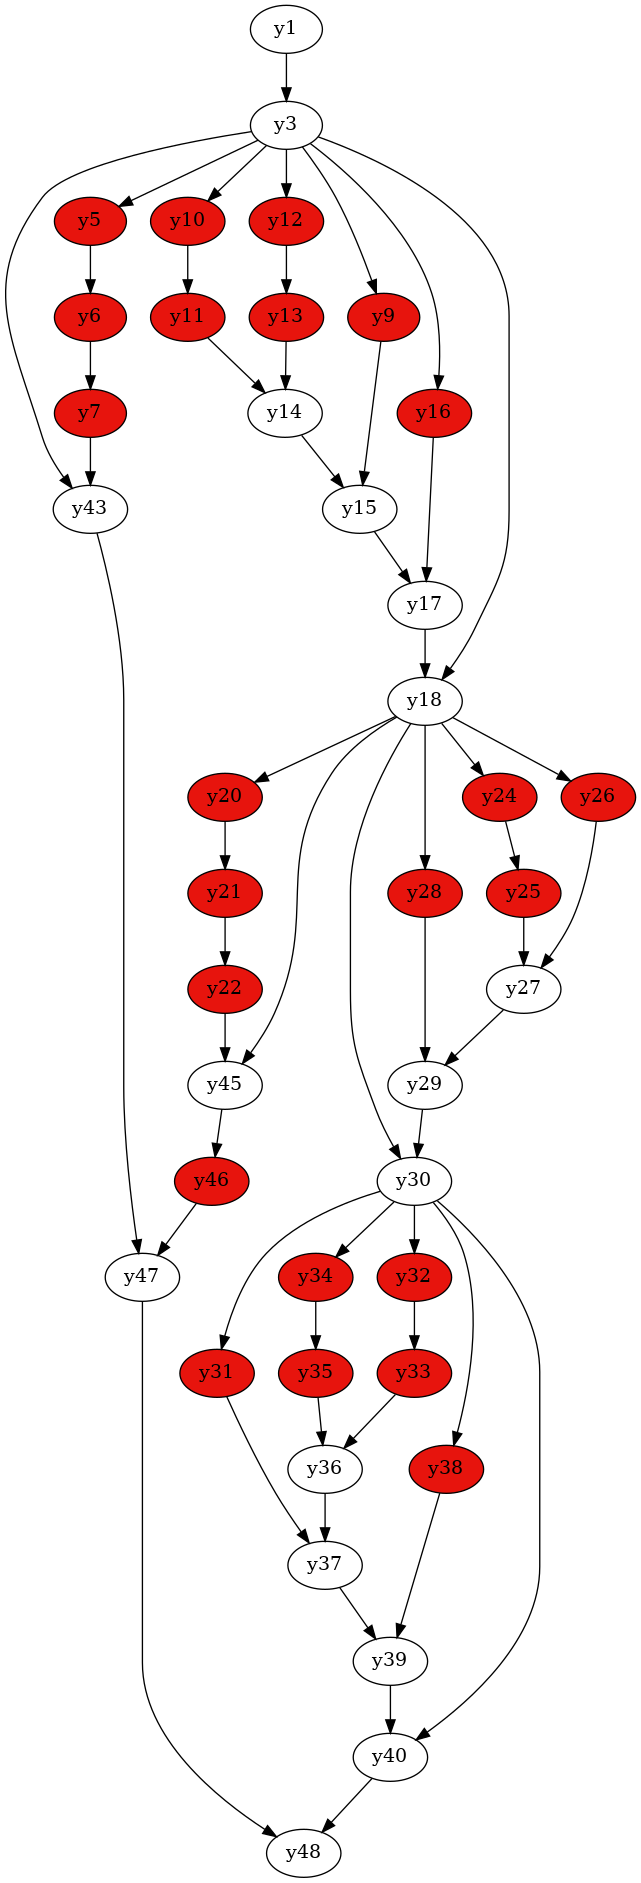
\includegraphics[width=\textwidth]{hash2if1.png}
\column{0.75\textwidth}
\begin{itemize}
  \item Стягивание вершин = подстановка термов
  \item Много вершин с outdeg = indeg = 1
  \item Можно их стянуть
\end{itemize}
\begin{megaalgorithm}\tiny
  \caption{\tiny contractions}
\begin{algorithmic}
  \State $(Y, P)\gets$ input
  \State $T \gets P(y_0, y_n)$
  \For{$i \gets 1$ to $|Y|$}
      \If{\textcolor{red}{$indeg(y_i) = 1$ and $outdeg(y_i) = 1$}}
          \For{$j \gets i + 1$ to $n$}
              \State $T_j \gets T_j [y_i := T_i]$
          \EndFor
          \State $P \gets P [y_i := T_i]$
          \State $Y \gets Y \setminus (y_i, T_i)$
      \EndIf
  \EndFor
  \State \Return {$basic\_strategy(Y, P)$}
\end{algorithmic}
\end{megaalgorithm}
\end{columns}
\end{frame}

\begin{frame}\frametitle{Графовые эвристики 2}
  \begin{columns}
  \column{0.25\textwidth}
  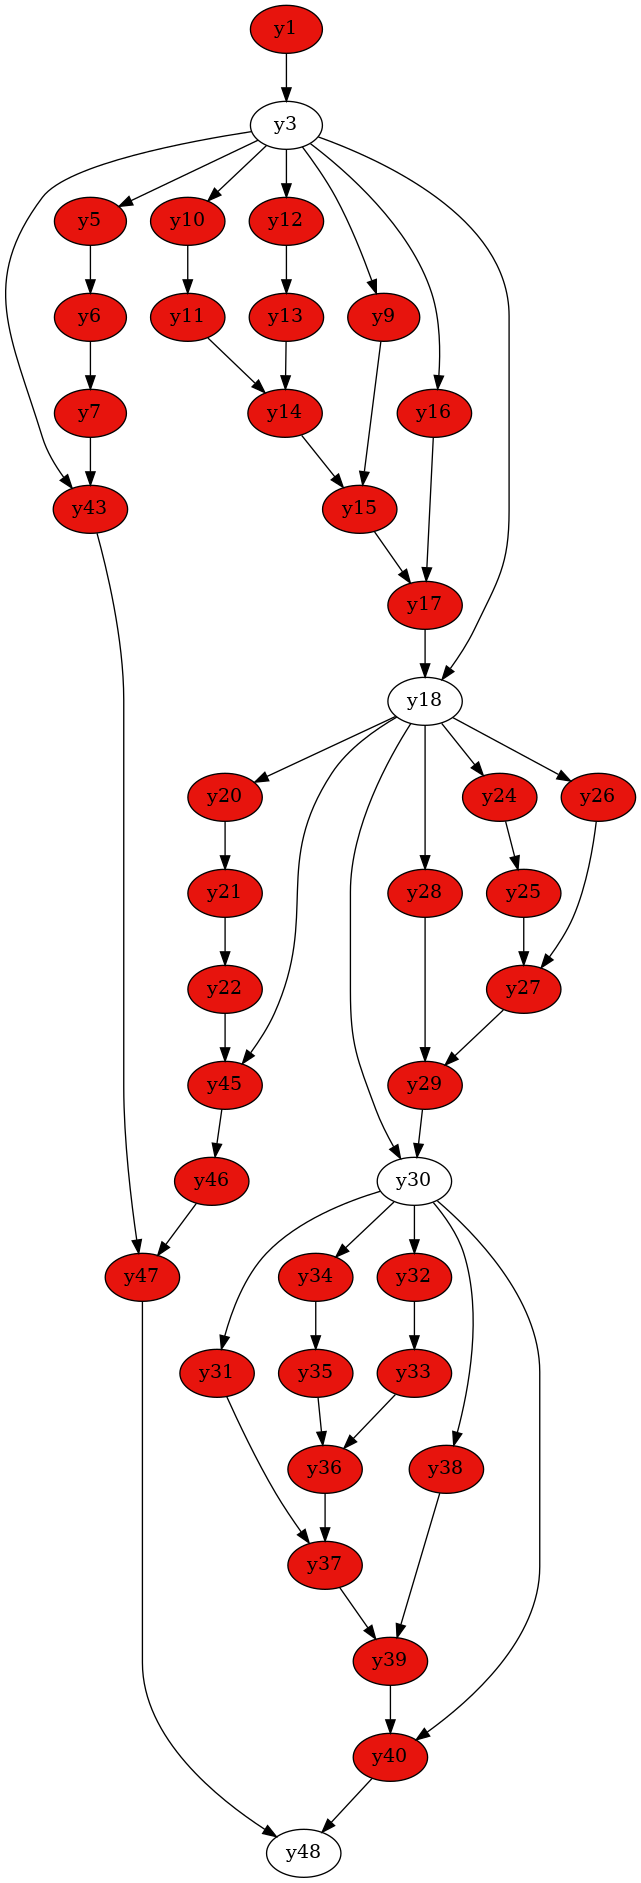
\includegraphics[width=\textwidth]{hash2if2.png}
  \column{0.75\textwidth}
  \begin{itemize}
    \item Почти все вершины с outdeg = 1
    \item Можно их стянуть
    \item От этого возникнет дубликация, но не очень большая
  \end{itemize}
\begin{megaalgorithm}\tiny
  \caption{\tiny contractions-strong}
\begin{algorithmic}
  \State $(Y, P)\gets$ input
  \For{$i \gets 1$ to $|Y|$}
      \If{\textcolor{red}{$outdeg(y_i) = 1$}}
          \For{$j \gets i + 1$ to $n$}
              \State $T_j \gets T_j [y_i := T_i]$
          \EndFor
          \State $P \gets P [y_i := T_i]$
          \State $Y\gets Y \setminus (y_i, T_i)$
      \EndIf
  \EndFor
  \State \Return {$basic\_strategy(Y, P)$}
\end{algorithmic}
\end{megaalgorithm}
  \end{columns}
  \end{frame}

\begin{frame}\frametitle{Эвристики на основе типов данных 1}
    \begin{columns}
    \column{0.25\textwidth}
    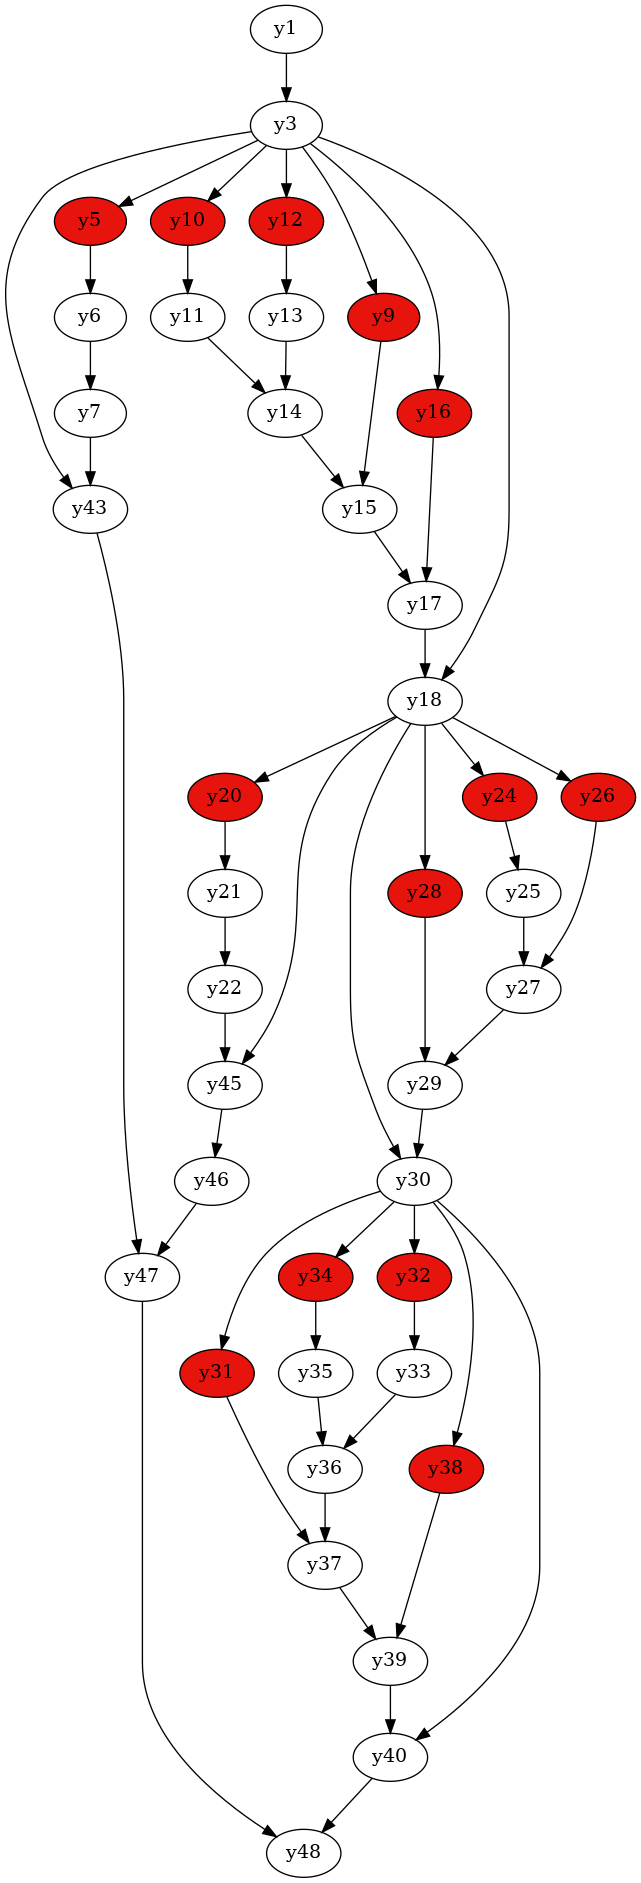
\includegraphics[width=\textwidth]{hash2if3.png}
    \column{0.75\textwidth}
    \begin{itemize}
      \item Определять indeg и outdeg сложно и долго
      \item Воспользуемся информацией о типах
      \item Все вершины типов LocalStateMapping и FieldType имеют indeg = outdeg = 1
    \end{itemize}
    \begin{megaalgorithm}\tiny
      \caption{\tiny contractions-typebased}
    \begin{algorithmic}
      \State $(Y, P)\gets$ input
      \For{$i \gets 1$ to $|Y|$}
          \If{\textcolor{red}{$typeof(y_i)$ is $LocalStateMapping$ or $FieldType$}}
              \For{$j \gets i + 1$ to $n$}
                  \State $T_j \gets T_j [y_i := T_i]$
              \EndFor
              \State $P \gets P [y_i := T_i]$
              \State $Y\gets Y \setminus (y_i, T_i)$
          \EndIf
      \EndFor
      \State \Return {$basic\_strategy(Y, P)$}
    \end{algorithmic}
  \end{megaalgorithm} 
    \end{columns}
\end{frame}

\begin{frame}\frametitle{Эвристики на основе типов данных 2}
  \begin{columns}
  \column{0.25\textwidth}
  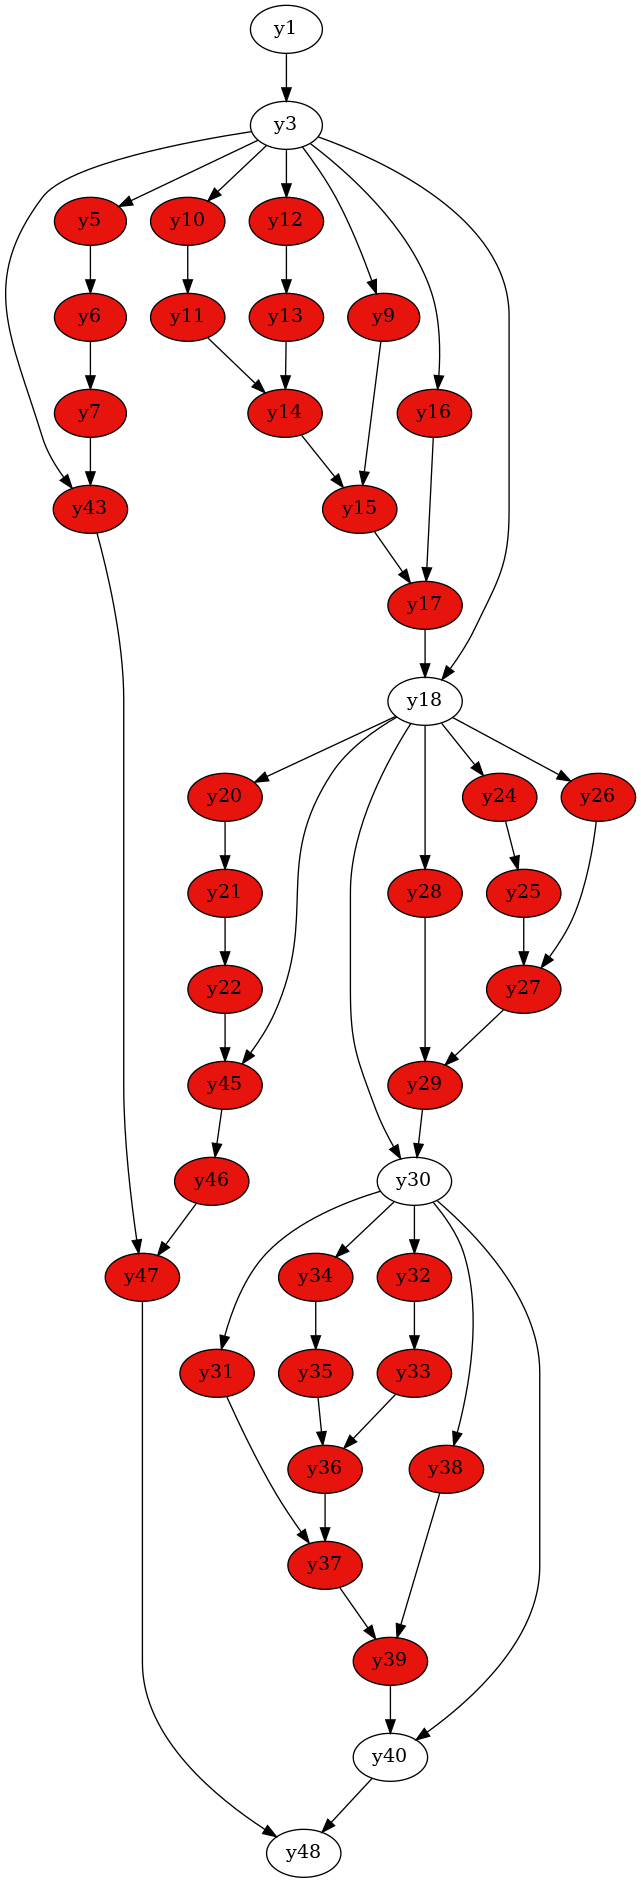
\includegraphics[width=\textwidth]{hash2if4.png}
  \column{0.75\textwidth}
  \begin{itemize}
    \item Вершины типа Ledger, как правило, имеют большой outdeg
    \item Почти все вершины других типов имеют outdeg = 1
  \end{itemize}
  \begin{megaalgorithm}\tiny 
    \caption{\tiny contractions-strong-typebased}
  \begin{algorithmic}
    \State $(Y, P)\gets$ input
    \For{$i \gets 1$ to $|Y|$}
        \If{\textcolor{red}{$typeof(y_i)$ is not $Ledger$}}
            \For{$j \gets i + 1$ to $n$}
                \State $T_j \gets T_j [y_i := T_i]$
            \EndFor
            \State $P \gets P [y_i := T_i]$
            \State $Y\gets Y \setminus (y_i, T_i)$
        \EndIf
    \EndFor
    \State \Return {$basic\_strategy(Y, P)$}
  \end{algorithmic}
\end{megaalgorithm}  
  \end{columns}
\end{frame}

\begin{frame}\frametitle{Сравнение. Бенчмарки}
  \begin{itemize}
    \item Синтетическая часть. Реализации алгоритма хеширования на языке Ursus, линейно увеличивающиеся по размеру кода
    \begin{itemize}
      \item Simple, линейный код
      \item Recursive, рекурсивный код
      \item \textcolor{gray}{If, линейный код с условными операторами}
      \item \textcolor{gray}{IfAndRecursion, рекурсивный код с условными операторами}
    \end{itemize}
    \item \textcolor{gray}{Реальная часть. Верификация смарт-контракта мультисиг-кошелька из практики компании Pruvendo}
  \end{itemize}
  \end{frame}

\begin{frame}\frametitle{Сравнение. bottomup}
\begin{itemize}
  \item TODO
  \item TODO
\end{itemize}
\end{frame}

\begin{frame}\frametitle{Сравнение. ??}
TODO
\end{frame}

\begin{frame}\frametitle{Сравнение. ??}
\begin{itemize}
  \item TODO
  \item TODO
\end{itemize}
\end{frame}

\begin{frame}\frametitle{Результаты}
\begin{itemize}
    \item TODO
    \item TODO
    \item TODO
    \item TODO
\end{itemize}
\end{frame}

\appendix
\backupbegin

\begin{frame}\frametitle{Apx 1}
TODO
\end{frame}

\backupend
\end{document}
